% \subsection{Performance} How does the languages compare in a
% performance benchmark?
% \begin{itemize}
% \item Benchmark of binomial pricer on expiry = 1,2,4,8,16,32,64,128 years.
% \item Benchmark of Longstaff and Schwartz
% \item Which optimizations are performed?
% \item How many in-code optimiser hints (inlining-statements, forcing
%   of delayed arrays etc.) are necessary to get decent performance?
% \item How does the performance of a naive implementation (no
%   optimiser hints) compare to an optimised version?
% \end{itemize}

\chapter{Evaluation of performance}
\label{chap:performance}
We will now look at how the different languages compare in
performance, by implementations of the cases described in Chapter
\ref{chap:cases}.


% We will start by taking a brief look at which
% optimisations are implemented in each language, and what we can
% expect.

% \section{Optimisations}

% \subsection{Deforestation}
% Stream fusion, program composition or deforestation is a technique
% that aims composing several functions into one to optimize away
% intermediate datastructures\footnote{which it what gives it the name
%   deforestation: intermediate tree structures are removed} and thus
% avoid expensive memory access.

% A simple example is that of computing sum of squares:
% \begin{verbatim}
% foldl (+) 0 (map (^2) xs)
% \end{verbatim}
% where the unoptimized program would have to write all the squared
% numbers into memory during the computation of map and then read back
% from memory during the summation. Fusing the \verb|map| into the
% \verb|foldl| avoids this intermediate array:
% \begin{verbatim}
% foldl (\a b -> a + b^2) 0 xs
% \end{verbatim}

% This optimization is at the heart of both the Nikola and Repa
% architectures, where it happens through the use of delayed
% arrays. Data.Vector also performs some stream fusion by employing GHC
% rewrite rules. Fusion is currently being implemented in
% Accelerate. The newest version on Hackage (0.12.1.0) does not perform
% any fusion, but the development repository contains a not completely
% functional implementation, so it will possibly be part of the next
% release.

% On GPU hardware this also means that several kernels can be merged
% into one, and the overhead involved in kernel launches can thus also
% be avoided.

% In CUDA this optimization must be done by hand \todo{Cite someone that
%   says nvcc doesn't provide deforestation/fusion}

% \subsection{Prefix sum, tree reduction}
% Accelerate comes with a number of built in parallel algorithms, that
% runs efficiently on GPUs. Such as

% \subsection{Strided memory access}
% Because of limited caches in GPUs, out of order memory access incurs a
% huge performance penalty. We must thus make sure that memory accesses
% inside GPU warps are coalesced.

% Accelerate guarantees this approach, as long as you use the built in
% high order functions, and avoid using the array lookup function
% \begin{verbatim}
% (!) :: (Shape ix, Elt e) => Acc (Array ix e) -> Exp ix -> Exp e
% \end{verbatim}

% \todo{Nikola??}

% \subsection{Limit branch divergence}
% Accelerate goes a long way to restrict the possible programs you can
% write, such that they can make certain performance guarantees. For
% instance, they do not allow you to write sequential loops running on
% the GPU as this may allow one thread to diverge letting the remaining
% threads in a block waiting. This is problematic, as certain problems
% are more efficiently expressed using nested loops, and you thus need
% to manually flatten, giving a performance penalty.

% Nikola on the other hand, does not make such limitations and lets the
% programmer himself evaluate \todo{complete this}

\section{Benchmark setup}
In our benchmarks we only measure the time used by each of the
different implementations. Other parameters, such as memory
consumption on host and device, have been left out. For GPU
implementations of the algorithms we can usually infer the device
memory consumption directly from the program, but an analysis of host
memory usage would have been interesting, but we had to limit
ourselves and thus deemed it outside our scope.

The benchmarks are made on programs written in an as idiomatic style
as we possible could, and if we have one available, we use a version
written by a language expert. We are not interested in comparing fully
optimized programs, as we want to measure how the languages compare in
performance when the languages are used as the language author inteded
it, and in a fashion appropriate for human reading. One exception is
though CUDA, where we want to compare our ``idiomatic'' versions to a
fully optimized CUDA implementation, employing all the tricks of the
trade.

The output of all our benchmarks has been verified manually, through
comparison of results with our reference $R$ implementations of the
algorithms.

\subsection{Hardware}
All benchmarks have been performed on a computer provided by the
HIPERFIT research center running Ubuntu 12.04 LTS and CUDA 5.0.

The hardware specifications is as follows:
\begin{itemize}
\item 2 $\times$ AMD Opteron\texttrademark\ 6274 processors (16 cores each, clocked at 2,2 Ghz)
\item 132 GB (approx. 126 GiB) main memory
\item Quad SLI consisting of two GeForce GTX 690 (each a dual-head
  GPU). See full specifications in Table \ref{tab:hardware}.
\end{itemize}
\begin{table}
\begin{minipage}[b]{0.50\linewidth}
  \centering
  \begin{tabular}{ll}
    Multiprocessors & $2 \times 8$ SMs\\
    Cores per SM & 192 cores \\
    CUDA cores & $2 \times 1536$ cores\\
    Clock rate & 915 Mhz \\
    Memory & $2 \times 2$ GB \\
    RAM technology & GDDR5 \\
    Memory bandwidth & $2 \times 192.3$ GB/s \\
    \hline
  \end{tabular}
  \caption{Geforce GTX 690 specification}
  \label{tab:hardware}
\end{minipage}
\begin{minipage}[b]{0.50\linewidth}
  \centering
  \begin{tabular}{cr}
    \textbf{Language} & \textbf{Time}  \\ \hline
    C & $67.03 \mu s$ \\
    R & $89.13 \mu s$ \\
    CUDA C & $66.23 \mu s$ \\
    Haskell & $107.45 \mu s$ \\ \hline
  \end{tabular}
  \caption{Benchmarking overhead}
  \label{tab:benchmarking-overhead}
\end{minipage}
\end{table}

Ideally, we would have evaluated all benchmarks on two different
systems, to make sure that our results are not specific to one
setup. We did however only have access to this one machine with CUDA
version 5.0 or newer, which was a required by the newest versions of
both Nikola and Accelerate.

\subsection{Software and compilation}
For each case, we have a set of different implementations and we want
to measure the time used by each implementation on varying problem
sizes. This was accomplished by developing a small benchmarking
tool\footnote{The tool is documented in the README available at
  \url{https://github.com/HIPERFIT/vectorprogramming/blob/master/README.md}}
that executed each experiment in succession, providing the input
through a small protocol over Unix standard I/O, and letting the
program respond with a result between each experiment. This response
was used to stop the time measurement.

Several of the libraries and languages we have used requires
individual compilation steps before the actual computation can take
place. We have decided not to include all initialization in the
running times, and only record the time used on the actual computation
and eventual memory allocation and memory transfers. This is done to make the
comparison fair, and because we think it is more important to optimize
the actual computation. Optimizing the compilation or interpretation
performance is also important, but we find that to be less of priority
now and it thus out of our current scope.

The benchmarking tool was developed using the Haskell
\texttt{criterion}\footnote{\url{http://hackage.haskell.org/package/criterion}}
package. Each experiment was been executed 100 times and the mean and
standard deviations was logged. To eliminate the possibility of errors
in our approach, we have measured the overhead involved in issuing a
request through standard I/O, by implementing an ``empty'' benchmark
in each language, and measured the time used on a just responding. The
results are shown in Table \ref{tab:benchmarking-overhead} (standard
deviations are not listed, but are in all cases negligible). The
significance of of course depends on the application, for most of our
purposes it is too small to make a difference, we will note when it
should be considered a source of error.

\section{Benchmarks}
We will now present the results of our benchmarks. We have two plots
for each benchmark: One showing the actual time used on each
computation, and one showing relative performances. All scales are
logarithmic.

\subsection{Benchmark 1: Binomial option pricing on the CPU}
\begin{figure}
	\centering
\begin{adjustbox}{minipage=1.3\textwidth,margin=0pt \smallskipamount,center}
	\subbottom[Speed-up relative to R implementation.]{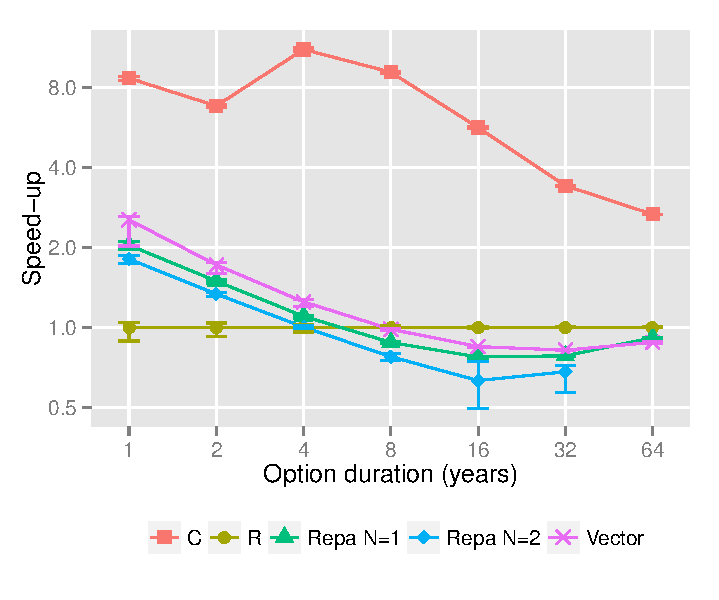
\includegraphics[width=0.5\textwidth]{graphics/final-benchmark/binomial-cpu/speedup-graph-final.pdf}\label{fig:binomial-cpu-speedup}
    \vspace{-12mm}}
  \subbottom[Absolute time usage.]{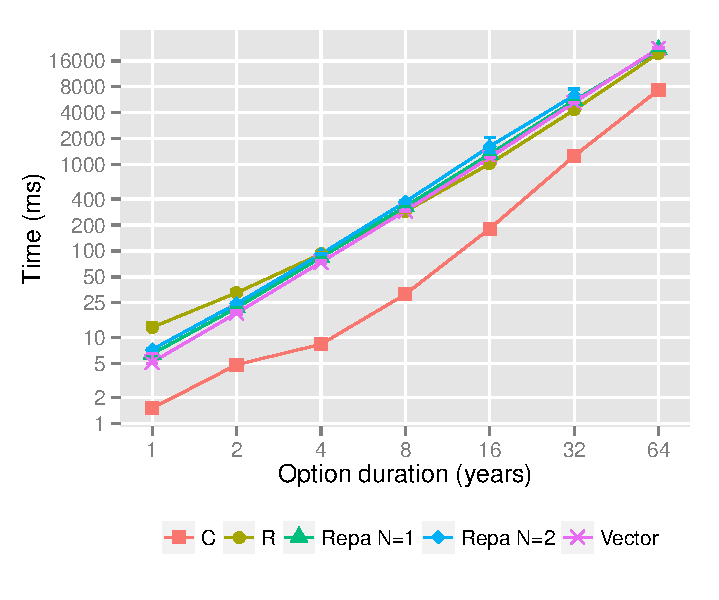
\includegraphics[width=0.5\textwidth]{graphics/final-benchmark/binomial-cpu/time-graph-final.pdf}\label{fig:binomial-cpu-time}}
\end{adjustbox}
\caption{Binomial option pricing (CPU).}
\label{fig:binomial-cpu}
\end{figure}

In our first benchmark we compare the performance of R and C languages
to the Repa and the \texttt{Data.Vector} Haskell libraries, on the
binomial option pricing case. All algorithms have been implemented
following Algorithm \ref{alg:binomial-algorithm}, in Section
\ref{sec:binomial-model}. The R and C implementations are equivalently
and are written by Rolf Poulsen, Professor of Financial Mathematics at
the Department of Mathematical Sciences, University of
Copenhagen\footnote{Obtained from
  \url{http://www.math.ku.dk/~rolf/FAMOES/}}. The \texttt{Data.Vector}
version and Repa implementations differ from these by not reusing
memory, and are thus not completely fair to Algorithm
\ref{alg:binomial-algorithm}, but using mutable arrays would not be
idiomatic in these library. The Repa version has been executed with
both one and two operating system threads (by setting the \texttt{+RTS
  -N} option).

The results are shown in Figure \ref{fig:binomial-cpu}. We see that
using an additional processor in Repa gives us a speed down. We have
also tested with additional processors, which performs even worse. The
amount of synchronization necessary between each iteration probably
the problem. It would be interesting to see how Repa would perform if
we were to execute it as a binomial pricer, but we have not had the
time to do that experiment.

We also see that the overhead incurred by reallocating arrays in each
iteration by the \texttt{Data.Vector} implementation is not that huge,
we could suspect that the garbage collectors liveness analysis detects
that we can reuse the just deallocated memory region.


\subsection{Benchmark 2: Binomial option pricing on the GPU}
\begin{figure}
	\centering
\begin{adjustbox}{minipage=1.3\textwidth,margin=0pt \smallskipamount,center}
	\subbottom[Speed-up relative to CUDA implementation.]{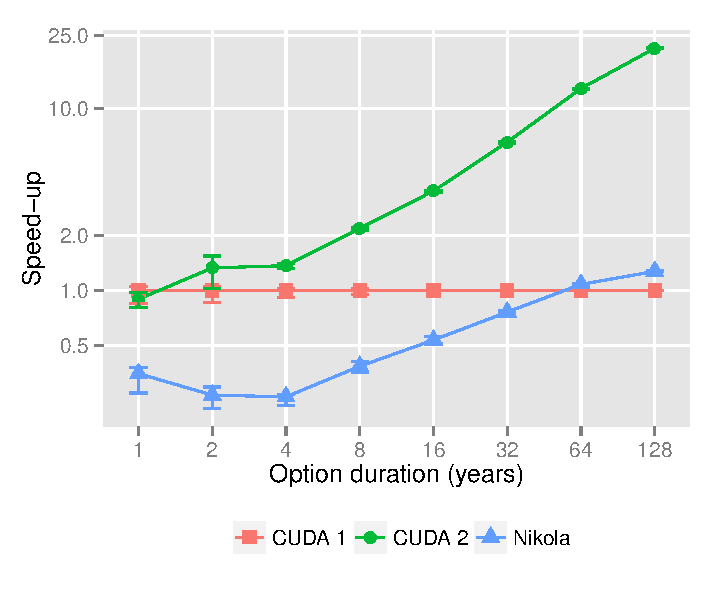
\includegraphics[width=0.5\textwidth]{graphics/final-benchmark/binomial-gpu/speedup-graph-final.pdf}\label{fig:binomial-gpu-speedup}}
	\subbottom[Absolute time usage.]{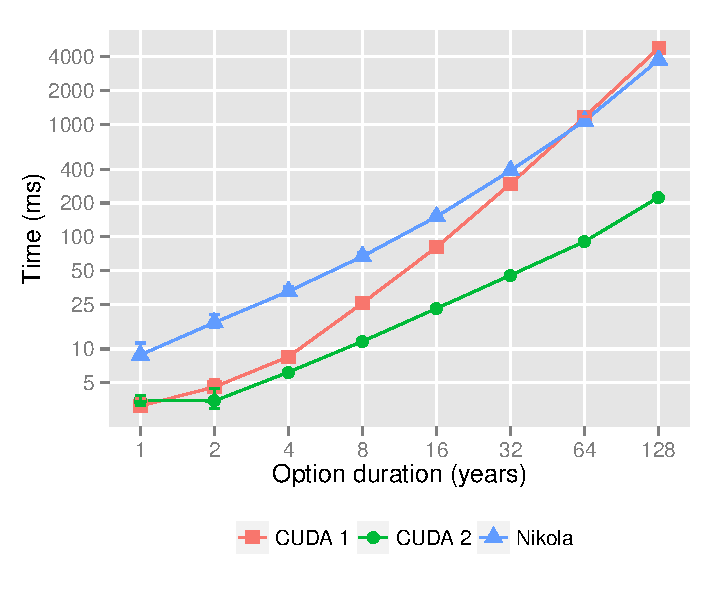
\includegraphics[width=0.5\textwidth]{graphics/final-benchmark/binomial-gpu/time-graph-final.pdf}\label{fig:binomial-gpu-time}}
\end{adjustbox}
  \caption{Binomial option pricing (GPU).}
\label{fig:binomial-gpu}
\end{figure}

In our second benchmark we compare the performance of Nikola, written
by the Nikola author Geoffrey Mainland, to two different CUDA
implementations of binomial option pricing. We also wished to
benchmark an Accelerate version, but we could not get a version to run
consistently and often it would break down with a CUDA error
(``unspecified launch failure``, which signals a memory access error
equivalent to a segmentation fault). The results are presented in
Figure \ref{fig:binomial-gpu}.

The first CUDA version is adapted from the portfolio pricer found in
NVIDIA's CUDA SDK, Algorithm \ref{alg:cuda-binom} in Section
\ref{sec:binomial-model}. This only runs on a single block and we see
that it is not competitive for long option durations. At options
running over 64 years ($16384$ time-steps), the Nikola
version outperforms it.

The second CUDA implementation is faster in all cases, except the
one-year option. We have written this version from scratch, and uses
all available cores to price the option. Synchronization happens by
returning to the CPU in each iteration, as we have to synchronize
across all blocks. The reason why it outperforms Nikola is perhaps
that the Nikola version does not reuse memory, and thus have to
reallocate and deallocate in each iteration, in all other aspects this
implementation is identical to the Nikola implementation.

\subsection{Benchmark 3: Sobol sequence generation on the CPU}
\begin{figure}
	\centering
  \begin{adjustbox}{minipage=1.3\textwidth,margin=0pt \smallskipamount,center}
	\subbottom[Speed-up relative to R implementation.]{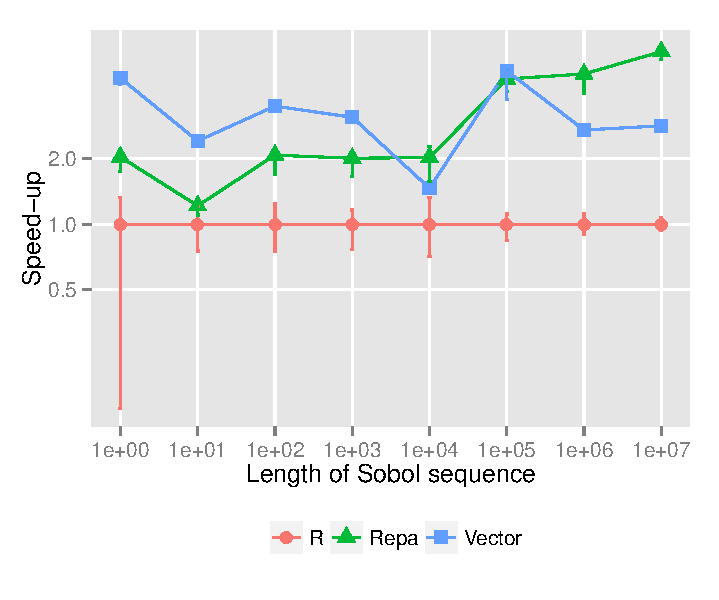
\includegraphics[width=0.5\textwidth]{graphics/final-benchmark/sobol-cpu/speedup-graph.pdf}\label{fig:sobol-cpu-speedup}}
	\subbottom[Absolute time usage.]{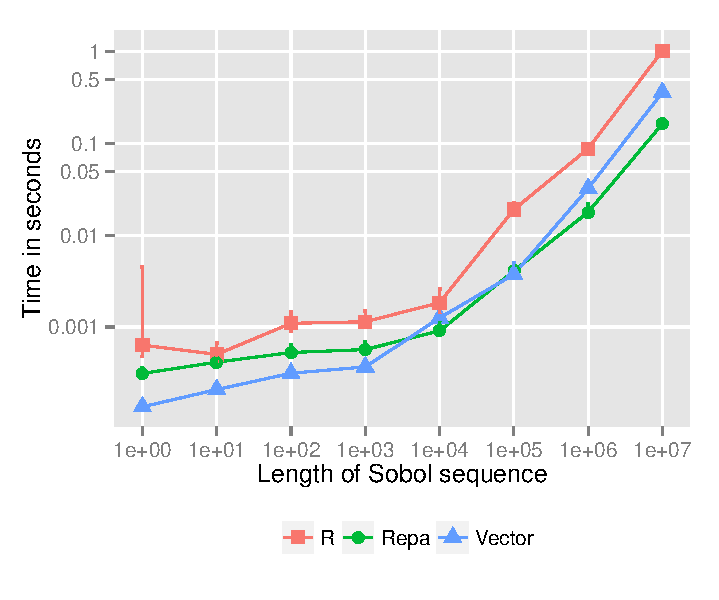
\includegraphics[width=0.5\textwidth]{graphics/final-benchmark/sobol-cpu/time-graph.pdf}\label{fig:sobol-cpu-time}}
\end{adjustbox}
  \caption{Sobol sequence generation (CPU).}
\label{fig:sobol-cpu}
\end{figure}

We now look at the performance of the Sobol sequence generators we
have implemented, and in this section we will concentrate on the CPU
versions implemented in R, Repa and \texttt{Data.Vector}. 

The R implementation is from the R-package \texttt{randtoolbox} which
interfaces with a Fortran implementation that uses the recursive
Algorithm \ref{alg:sobol-recursive}, Section \ref{sec:sobol}. This is
also the algorithm we have implemented in \texttt{Data.Vector}, but in
Repa we have used \todo{Arg! Latest results are from the wrong
  Repa-version! And we don't know the number of cores used in previous
  executions.}

The results are presented in Figure \ref{fig:sobol-cpu}.

\subsection{Benchmark 4: Sobol sequence generation on the GPU}
\begin{figure}
	\centering
\begin{adjustbox}{minipage=1.3\textwidth,margin=0pt \smallskipamount,center}
	\subbottom[Speed-up relative to CUDA implementation.]{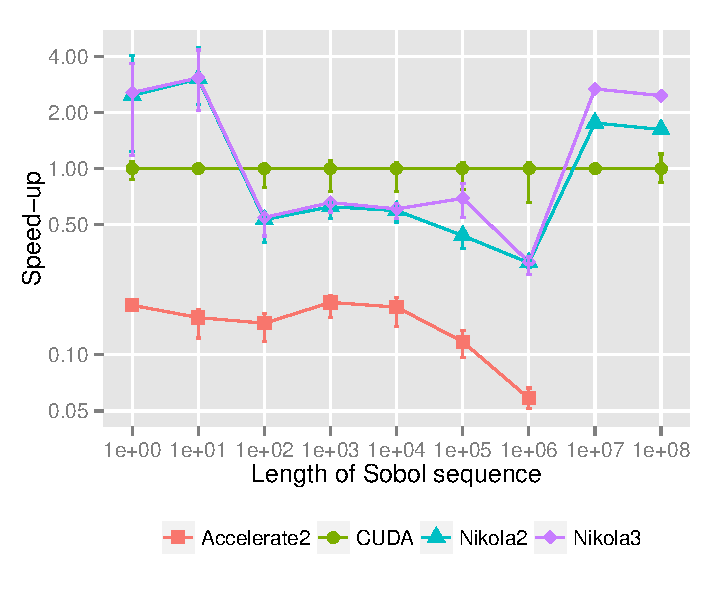
\includegraphics[width=0.5\textwidth]{graphics/final-benchmark/sobol-gpu/speedup-graph-final.pdf}\label{fig:sobol-gpu-speedup}}
	\subbottom[Absolute time usage.]{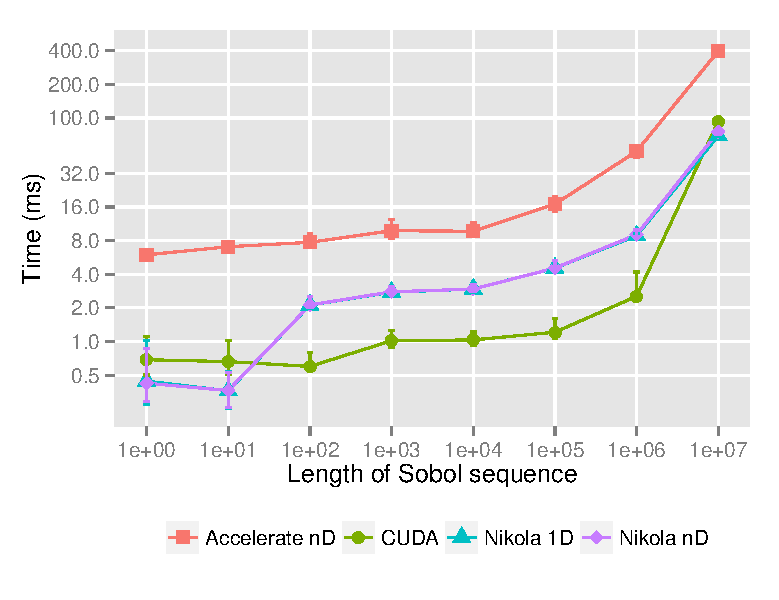
\includegraphics[width=0.5\textwidth]{graphics/final-benchmark/sobol-gpu/time-graph-final.pdf}\label{fig:sobol-gpu-time}}
\end{adjustbox}
  \caption{Sobol sequence generation (GPU).}
\label{fig:sobol-gpu}
\end{figure}

For GPUs, we have Sobol sequence generation implementations in
Accelerate, CUDA in addition to two Nikola variants. The results are
presented in Figure \ref{fig:sobol-gpu}. 

\subsection{Benchmark 5: Longstaff and Schwartz option pricing on the CPU}
\begin{figure}
	\centering
\begin{adjustbox}{minipage=1.3\textwidth,margin=0pt \smallskipamount,center}
	\subbottom[Speed-up relative to R implementation.]{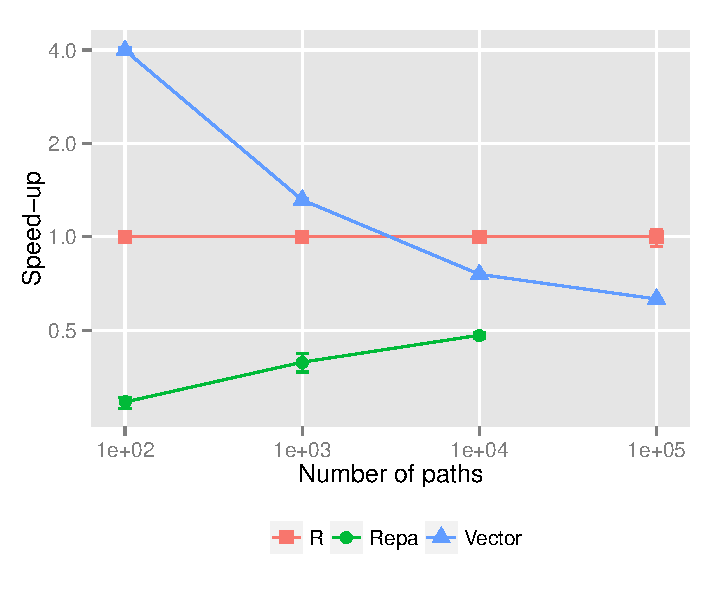
\includegraphics[width=0.5\textwidth]{graphics/final-benchmark/lsm-cpu/speedup-graph-final.pdf}\label{fig:lsm-cpu-speedup}}
	\subbottom[Absolute time usage.]{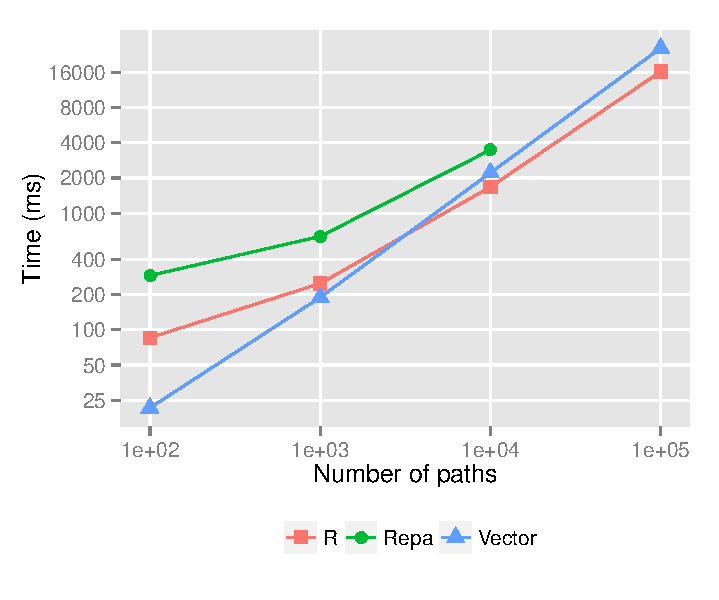
\includegraphics[width=0.5\textwidth]{graphics/final-benchmark/lsm-cpu/time-graph-final.pdf}\label{fig:lsm-cpu-time}}
\end{adjustbox}
  \caption{Longstaff \& Schwartz option pricing (CPU).}
\label{fig:lsm-cpu}
\end{figure}

We did only have time to implement Longstaff and Schwartz on the
CPU. \todo{why not Accelerate and Nikola}


% Speed up graph. In the graph we use the sequential version written
% with Data.Vector as a baseline for the comparison.

% Accelerate is not included, because of problems in their stream fusion
% algorithm leading to running times that evolve
% exponentially. Disabling fusion lead to CUDA exceptions.

% We see that the overhead incurred by using Nikola makes both
% sequential implementations (R and Data.Vector) faster for the smallest
% cases, and only when we reach the largest example (128 years expiry
% time) Nikola catches up.

% Repa is the best performing, even though it does not perform any GPU
% computations. We are not sure why Repa gives so varied speed-ups for
% different input sizes, but it might be because of our somewhat
% arbitrary threshold for which problem sizes should be executed in
% parallel and which should be executed sequentially.


%%% Local Variables:
%%% mode: latex
%%% TeX-master: "../master"
%%% End:
